\documentclass[english,dvipdfmx]{jsarticle}
\usepackage{amsmath,amssymb}
\usepackage{color}
\usepackage[hiresbb]{graphicx}
\usepackage{here}
\newcommand{\average}[1]{\ensuremath{\langle#1\rangle} }
\newcommand*{\point}{\textcircled{\textcolor{red}{\scriptsize キ}}}
\newcommand*{\proof}{\textcircled{\textcolor{blue}{\scriptsize P}}}
\begin{document}
\section{Binary Relation}
\begin{description}
    \item[\bf{Definition:}] Equivalence relation $R \subset X \times X$ on a set $X$ \\
    \point : 等号関係の一般化
    \begin{equation*} \begin{cases}
        \text{Reflexivity} : \quad &xRx \quad ( \forall x \in X )  \\
        \text{Symmetry} : \quad  &xRy \Rightarrow yRx \quad ( \forall x,y \in X ) \\
        \text{Transitivity} : \quad &xRy , yRz \Rightarrow xRz \quad (\forall x,y,z \in X )
    \end{cases} 
    \end{equation*}
    \item[\bf{Example:}] An example of relation $R$
    \begin{enumerate}
        \item $ = $
        \item congruence, similarity (geometry)
        \item $x \equiv y \quad (mod \ p)$
    \end{enumerate} 
    \item[\bf{Definition:}] Equivalence class
    \begin{equation*}  
        [a] = \{ x \in X \ | \ xRa \} \quad ( a \in X , R : \text{relation on a set } X )
    \end{equation*}
    \item[\bf{Definition:}] Quotient space \\
    \textcircled{\textcolor{red}{\scriptsize キ}} : 同値類集合の集合
    \begin{equation*} 
    X / R = \{ [a] \ | \ a \in X \} 
    \end{equation*}
    \item[\bf{Definition:}] Natural projection (Quotient mapping)
    \begin{equation*} 
    \gamma : X \longmapsto X / R ,\ \gamma(x) = [x] \quad ( x \in X )
    \end{equation*}
    \item[\bf{Definition:}] \textcolor{red}{order} relation $R \subset X \times X$ on a set $X$ $( xRy \Leftrightarrow x\leq y)$ \\ 
    \point : 大小関係の一般化
    \begin{equation*}
    \begin{cases}
        \text{Reflexivity} : \quad &x\leq x \quad ( \forall x \in X )  \\
        \text{\color{red} Antisymmetry} : \quad  &x\leq y ,y\leq x \Rightarrow x=y \quad ( \forall x,y \in X ) \\
        \text{Transitivity} : \quad &x\leq y , y\leq z \Rightarrow x\leq z \quad (\forall x,y,z \in X )
    \end{cases}
    \end{equation*}
    \item[\bf{Definition:}] Ordered set $(X , \leq)$ \\
        $\leq \text{ is order relation on a set }X$ 
    \item[\bf{Example:}] An example of ordered set
    \begin{enumerate}
        \item $ (\mathbb{R},\leq) $ , $ (\mathbb{R},<) $ is not ordered set
        \item $ ( 2^X,\subset) $
    \end{enumerate}
    \item[\bf{Definition:}] Ordered subset $(M,\leq_M) \subset (X, \leq)$
    \begin{equation*} 
        M \subset X , a \leq_M b \Leftrightarrow a \leq b
    \end{equation*}
    \item[\bf{Definition:}] Partial order and total order
    \begin{eqnarray*} 
        \exists (x,y) \in R \quad ( x,y \in X ) &\Rightarrow& R \text{ is partial order} ,\ (X , R) \text{ is partially ordered set} \\
        \forall (x,y) \in R \quad ( x,y \in X ) &\Rightarrow& R \text{ is total order} ,\ (X , R) \text{ is totally ordered set}
    \end{eqnarray*}
\end{description}
\newpage
\section{Partially Order Set}
\begin{description}
    \item[\bf{Definition:}] Maximum (minimum) , supremum (infimum) and upper bound (lower bound)
    \begin{eqnarray*}
    \max \ A = {\color{red}M}  &\Leftrightarrow& a \leq {\color{red}M} \quad ( {\color{red}M} \in A ,\ \forall a \in A )  \\
    {\color{red}{s}} \text{ is one of upper bounds of } A &\Leftrightarrow& a \leq {\color{red}{s}} \quad ( \forall a \in A ) \\
    \sup \ A = {\color{red}M'} &\Leftrightarrow& \min \ S = {\color{red}M'} \quad ( S \text{ is a set of upper bounds of }A ) \\
    &\Leftrightarrow& \begin{cases}  \forall a \in A  ,\ a \leq {\color{red}M'} \\ \forall \epsilon > 0 ,\ \exists a \in A \ \text{s.t.} \ {\color{red}M'} - \epsilon < a \end{cases}
    \end{eqnarray*}
    \item[\bf{Example:}] An example of partially ordered set. $ \{ y \} \leq \{ x,z \} $ is not defined. \\
        \begin{minipage}{.4\textwidth}
            \centering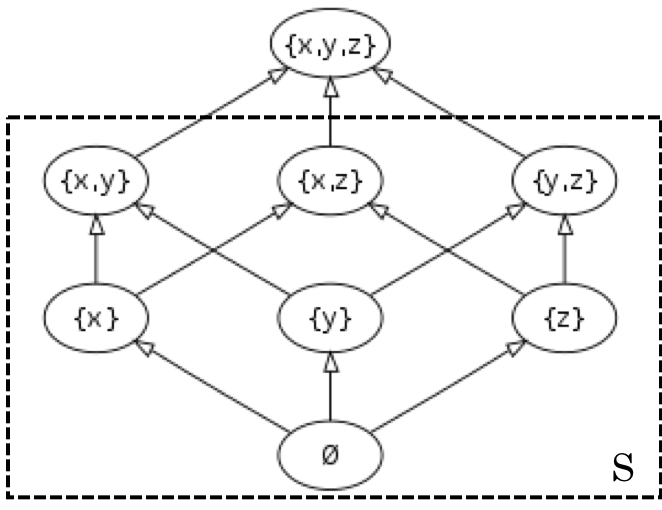
\includegraphics[width=7cm]{./set.png}
            \end{minipage}
            \hfill
            \begin{minipage}{.4\textwidth}
        $\max \ S$ : $None$ , $\min \ S$ : $\phi$\\
        $\sup \ S$ : $\{ x,\ y,\ z \}$ , $\inf \ S$ : $\phi$
        \end{minipage}
    \item[\bf{Theorem:}] Maximum, minimum, supremum and infimum exists uniquely.\\
        \proof : 最大値, 最小値の一意性は順序関係の反対称律を使う. \\
        \proof : 極大値, 極小値の一意性は最大値,最小値の一意性を使う.
    \item[\bf{Theorem:}] If maximum (minimum) of $A$ exists, $\max \ A = \sup \ A$ ($\min \ A = \inf \ A$ ). \\
        \proof : $\sup(\inf)$ の2つめの定義を使う.
    \item[\bf{Axiom:}] {\color{cyan}{Existance of supremum and infimum}}
        \begin{eqnarray*}
            & &A \subset \mathbb{R},\ A \neq \phi \\
            & &A \text{ is bounded above } \Rightarrow \sup \ A \text{ exists.} \\
            & &A \text{ is bounded below } \Rightarrow \inf \ A \text{ exists.}
        \end{eqnarray*}
    \item[\bf{Definition:}] Complete lattice \\
        a partially ordered set $X$ in which $\forall X' \subset X,\ X'$ have both $\sup \ X',\ \inf \ X'.$
\end{description}
\newpage
\section{Sequence}
    \begin{description}
        \item[\bf{Definition:}] Sequence is a mapping $ x : \mathbb{N} \longmapsto X $
        \item[\bf{Definition:}] Subsequence is a composite mapping $ x \circ \iota : \mathbb{N} \longmapsto X$ \\
        let $\iota : \mathbb{N} \longmapsto \mathbb{N} $ be the mapping where $ i \leq j \Rightarrow \iota(i) \leq \iota(j) $
        \item[\bf{Example:}] Overview of Sequence and Subsequence 
            \begin{figure}[H]
                \begin{center}
                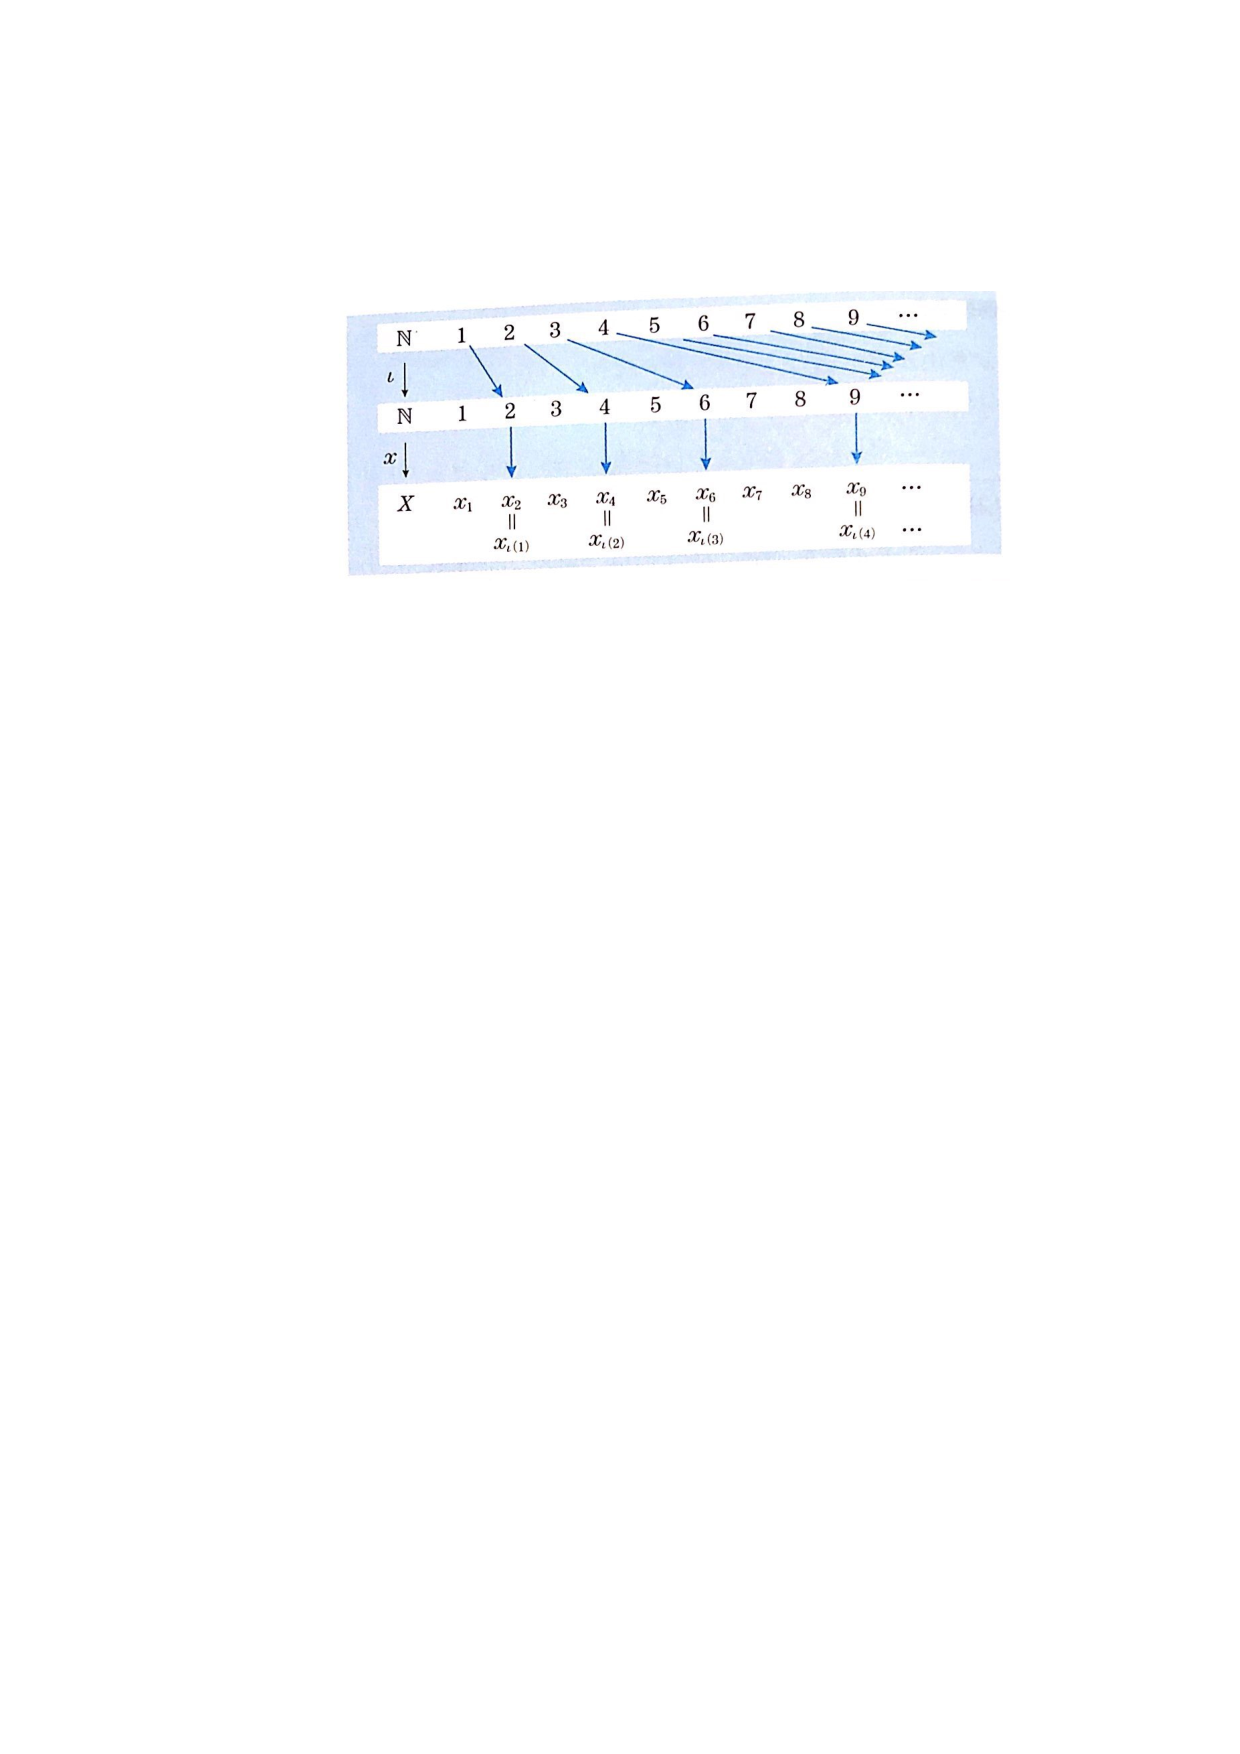
\includegraphics[clip,width=10cm]{./sequence.pdf}
                \caption{Sequence}
                \end{center}
            \end{figure}
        \item[\bf{Definition:}] Limit of sequence \\
            We call $\alpha$ the limit of the sequence $\{ x_n \}$ if the following condition holds:
            \begin{equation*}
                \forall \epsilon > 0 ,\ \exists N \in \mathbb{N} \text{ s.t. } n \geq N \Rightarrow | x_n - \alpha | < \epsilon
            \end{equation*}
        \item[\bf{Definition:}] 'bounded above', 'bounded below' \\
            The sequence $\{ x_n \}$ is 'bounded above' if the following condition holds:
            \begin{equation*}
                \exists M \in \mathbb{R},\ \forall i \in \mathbb{N},\ x_i \leq M
            \end{equation*}

        \item[\bf{Definition:}] Cauchy Sequence \\
            \point : 十分大きな$N \in \mathbb{N}$を選ぶと$n,\ m \geq N$において$x_n$と$x_m$の差をいくらでも小さくできる列. \\
            We call $\{ x_n \}$ a Cauchy Sequence if the following condition holds: 
            \begin{equation*}
                \forall \epsilon > 0,\ \exists N \in \mathbb{N} \text{ s.t. } n,\ m \geq N \Rightarrow | x_n - x_m | < \epsilon
            \end{equation*}
        \item[\bf{Example:}] An exapmle of Cauchy Sequence \\
            %% TODO Cauchy Sequence の 例 を書く. 証明をすること.
        \item[\bf{Theorem:}] If $\{ x_n \} ,\ \{ y_n \}$ are Cauchy Sequences, 
            \begin{equation*}
                \{ x_n + y_n \} ,\ \{ x_n \cdot y_n \} \text{ are Cauchy Sequences.} 
            \end{equation*}
        \item[\bf{Theorem:}] If a sequence $x_n$ converges to some limit, $x_n$ is a Cauchy Sequence.
        \item[\bf{Theorem:}] If a sequence $x_n$ is a Cauchy Sequence, $x_n$ is bounded.
    \end{description}

\newpage
\section{Real Number}
    \subsection{Definition of $\mathbb{N}$ and Construction of $\mathbb{Z},\ \mathbb{Q}$}
    \begin{description}
        \item[\bf{Axiom:}] Peano axioms \\
        \point : 自然数の定義 \\
        Define $S$ as a single-vlued successor function. (ex. $S(1) = 2$ )
        \begin{enumerate}
            \item $0$ is a natural number.
            \item For every natural number $n$, $S(n)$ is a natural number.
            \item For every natural number $n$, $S(n) = 0$ is false.
            \item $a,\ b \in \mathbb{N},\ a \neq b \Rightarrow S(a) \neq S(b)$
            \item if $\Phi$ is a unary preficate such that: 
                \begin{itemize}
                    \item $\Phi(0)$ is true.
                    \item for every natural number $n$, $\Phi(n)$ being true implies that $\Phi(S(n))$ is true.
                \end{itemize}
                ( \bf{Mathematical induction} )
        \end{enumerate}
        \item[\bf{Definition:}] Integers and rational number
            \begin{equation*}  
            \mathbb{Z} = \mathbb{N} \cup -\mathbb{N} ,\ \mathbb{Q} = \{ \frac{b}{a} \mid a,\ b \in \mathbb{Z},\ a \neq 0 \}
            \end{equation*}
    \end{description}
    \subsection{Construction of $\mathbb{R}$}
    \subsubsection{Dedekind cut}
    \begin{description}
    \item[\bf{Definition:}] Dedekind cut of $\mathbb{Q}$
        \begin{equation*}
            A \cup B = \mathbb{Q},\ A \cap B = \phi,\ A \neq \phi,\ B \neq \phi,\ a \in A,\ b \in B \Rightarrow a < b
        \end{equation*}
    \item[\bf{Definition:}] Real number $\alpha$ is defined as a boundary value $\alpha = \average{A \mid B}$ of Dedekind cut. \\
        \point : 有理数全体集合のデデキント切断の境界値を実数と定義.
    \end{description}
    \subsubsection{Completion of rational numbers via Cauchy sequences}
    \begin{description}
    \item[\bf{Definition:}] Equivalence relation of Cauchy sequences
        \begin{eqnarray*}
            \{ a_n \} \sim \{ b_n \} &\Leftrightarrow& \lim_{n \to \infty} a_n = \lim_{n \to \infty} b_n = \alpha \\
            &\Leftrightarrow& \forall \epsilon > 0,\ \exists N \in \mathbb{N} \text{ s.t. } n \geq N \Rightarrow | a_n - b_n | < \epsilon
        \end{eqnarray*}
    \item[\bf{Definition:}] $\mathbb{R}$ \\
        We can define the bijection $ \Phi : (S \ / \sim) \longmapsto \mathbb{R} \quad ( S \text{ is the set of all Cauchy Sequences on }\mathbb{Q} ) $
        \begin{equation*}
            \Phi( [\{ a_n \}] ) = \lim_{n \to \infty} a_n \in \mathbb{R}
        \end{equation*}
        \point : $\mathbb{Q}$上のコーシー列の同値類と実数の間に1対1写像を定義する.
        \item[\bf{Example:}] Napier's constant $e = \displaystyle \lim_{n \to \infty} ( 1 + \frac{1}{n} )^n ,\ a_n = (1 + \frac{1}{n})^n\text{ is a Cauchy Sequence.}$ 
    \end{description}
    \subsection{Continuity of real numbers}
    \subsubsection{The Density of the Rational Numbers / The Density of the Irrational Numbers}
        %% TODO 証明をきちんと追っておくこと.
        \begin{description}
            \item[\bf{Theorem:}] The Density of the Rational Numbers
                \begin{equation*}
                    \forall x,\ y \in \mathbb{R},\ x < y \Rightarrow \exists r \in \mathbb{Q} \text{  s.t. } x < r < y
                \end{equation*}
                ※ Another expression : $ \forall \epsilon > 0 ,\ a \in \mathbb{R} ,\ \exists r \in \mathbb{Q},\ | a - r | < \epsilon $
            \item[\bf{Theorem:}] The Density of the Irrational Numbers
                \begin{equation*}
                    \forall x,\ y \in \mathbb{R},\ x < y \Rightarrow \exists q \in \mathbb{R} \backslash \mathbb{Q} \text{  s.t. } x < q < y
                \end{equation*}
            \item[\bf{Theorem:}] Archimedean property \\
                \point : 有理数の稠密性と同値 
                \begin{equation*}
                    \forall a,\ b \in \mathbb{R},\ 0 < a < b \Rightarrow \exists n \in \mathbb{N} \text{ s.t. } b < na
                \end{equation*}
            \item[\bf{Theorem:}] $\mathbb{N} \subset \mathbb{R}$ is not bounded above. \\
                \point : 有理数の稠密性と同値
            \item[\bf{Theorem:}] $lim_{n \to \infty} \frac{1}{n} = 0$ \\
                \point : 有理数の稠密性と同値
        \end{description}
    \subsubsection{Completeness of the real numbers}
        \begin{description}
            \item[\bf{Axiom:}] Every Cauchy Sequence on $\mathbb{R}$ is convergent. \\
            \point : 一般 : 収束列 $\Rightarrow$ Cauchy列, $\mathbb{R}$ : 収束列$\Leftrightarrow$ Cauchy列.
            \item[\bf{Axiom:}] カントールの区間縮小定理
                %%  TODO カントールの区間縮小定理を理解する. 
        \end{description}
    \subsubsection{Dedekind Theorem}
    \point : 4.3.1 \& 4.3.2 と同値.
    \begin{description}
        \item[\bf{Definition:}] Dedekind cut of $\mathbb{R}$
            \begin{equation*}
                A \cup B = \mathbb{R},\ A \cap B = \phi,\ A \neq \phi,\ B \neq \phi,\ a \in A,\ b \in B \Rightarrow a < b
            \end{equation*}
        \item[\bf{Axiom:}] {\color{cyan}{Dedekind theorem}} ( $\Leftrightarrow$ continuity of real numbers ) \\
            For any cut $\average{A \mid B}$ of the set of real numbers there exists only one real number $\gamma$ s.t:
            \begin{equation*}
                \alpha \in A ,\ \beta \in B \Rightarrow \alpha \leq \gamma \leq \beta ,\ \gamma \text{ is } {\color{red}{\max \ A}} \text{ or } {\color{red}{\min \ B}}
            \end{equation*}
    \end{description}
    %%  TODO 以下を理解する. 
    \subsubsection{単調有界数列の収束}
    \subsubsection{ボルツァーノ-ワイアシュトラウスの定理}

\newpage
\section{Cardinality}
    \begin{description}
        \item[\bf{Definition:}] The cardinality of a set $A$ is denoted by $|A|,\ card \ A ,\ \# A $ etc...
            \begin{equation*}
                |A| = 
                \begin{cases}
                    \ n \in \{ 0 \} \cup \mathbb{N} &: \text{cardinality of finite set } \\
                    \ (others) &: \text{cardinality of infinite set} \quad ex.
                    \begin{cases}
                        \ \aleph_0 &: \text{ cardinality of countably finite set } \\
                        \ \aleph &: \text{ cardinality of the continuum }
                    \end{cases}
                \end{cases}
            \end{equation*}
        \item[\bf{Definition:}] $|A| = |B| \Leftrightarrow A \sim B \Leftrightarrow \exists f \text{ (a bijection function) } : A \longmapsto B $ \\
            $ R = \{ (A,B) \mid |A| = |B| \ \} \subset S \times S$ on a set $S$ is an equivalence relation. 
        \item[\bf{Definition:}] $|A| \leq |B|  \Leftrightarrow \exists f \text{ (a injective function) } : A \longmapsto B $ \\
            $ R = \{ (A,B) \mid |A| \leq |B|  \} \subset S \times S$ on a set $S$ is an order relation. \\
            \proof : 反対称律はBernsteinの定理を用いる.
        \item[\bf{Theorem:}] $ \aleph_0 < \aleph $ \\
            \proof : $ \mathbb{N} \not\sim  [ 0, 1 )$ をカントールの対角線論法で示す.
        \item[\bf{Theorem:}] $ |X| < |\mathfrak{P}(X)| $ \\
            \proof : $X \subset \mathfrak{P}(X)$より, $|X| \leq |\mathfrak{P}(X)|$は明らか.$|X| \not= |\mathfrak{P}(X)|$を対角線論法で示す.
        \item[\bf{Theorem:}] $A \cap B = \phi$ とする.
            \begin{enumerate}
                \item $\cup$
                    \begin{equation*}
                        | A \cup B | = | A | + | B | 
                    \end{equation*}
                    \begin{table}[H]
                        \begin{center}
                        \begin{tabular}{|c|c|c|c|} \hline
                            $|A \cup B| $& finite & countable & uncountable \\ \hline
                            finite & finite &  countable & uncountable \\ \hline
                            countable &  & countable & uncountable \\ \hline
                            uncountable & & & uncountable \\ \hline
                        \end{tabular}
                    \end{center}
                    \end{table}
                \item $\times$
                    \begin{equation*}
                        | A \times B | = | A | \cdot | B | 
                    \end{equation*}
                    \begin{table}[H]
                        \begin{center}
                        \begin{tabular}{|c|c|c|c|} \hline
                            $|A \times B| $& finite & countable & uncountable \\ \hline
                            finite & finite &  countable & uncountable \\ \hline
                            countable &  & countable & uncountable \\ \hline
                            uncountable & & & uncountable \\ \hline
                        \end{tabular}
                    \end{center}
                    \end{table}
                \item $pow$
                    \begin{equation*}
                        | A^B | = | A |^{| B |}
                    \end{equation*}
                    \begin{table}[H]
                        \begin{center}
                        \begin{tabular}{|c|c|c|c|} \hline
                            $|A^B| $& finite & countable & uncountable \\ \hline
                            finite & finite &  \textcolor{red}{uncountable} & uncountable \\ \hline
                            countable & countable & \textcolor{red}{uncountable} & uncountable \\ \hline
                            uncountable & uncountable & uncountable & uncountable \\ \hline
                        \end{tabular}
                    \end{center}
                    \end{table}
            \end{enumerate}
        \item[\bf{Example:}]
            \begin{equation*}
                A = \{ 1,\ 2,\ 3 \} ,\ |A| = 3
            \end{equation*}
            \begin{equation*}
                \aleph_0 = | \mathbb{N} | = | \mathbb{N}^2| = | \mathbb{Z} | = | \mathbb{Q} |
            \end{equation*}
            \begin{eqnarray*}
                \aleph &=& | \mathbb{R} | = | [a,b] | = | (a,b) | = | [a,b) | \\
                &=& \aleph_1 = |\mathfrak{P}(\mathbb{N})| \quad ( \text{ZFC Axioms} )
            \end{eqnarray*}
    \end{description}
\end{document}
